%%%%%%%%%%%%%%%%%%%%%%%%%%%%%%%%%%%%%%%%%%%%%%%
%
% Template per Elaborato di Laurea
% DISI - Dipartimento di Ingegneria e Scienza dell’Informazione
%
% update 2015-09-10
%
% Per la generazione corretta del 
% pdflatex nome_file.tex
% bibtex nome_file.aux
% pdflatex nome_file.tex
% pdflatex nome_file.tex
%
%%%%%%%%%%%%%%%%%%%%%%%%%%%%%%%%%%%%%%%%%%%%%%%

% formato FRONTE RETRO
\documentclass[epsfig,a4paper,11pt,titlepage,twoside,openany]{book}
\usepackage{epsfig}
\usepackage{plain}
\usepackage{setspace}
\usepackage[paperheight=29.7cm,paperwidth=21cm,outer=1.5cm,inner=2.5cm,top=2cm,bottom=2cm]{geometry} % per definizione layout
\usepackage{titlesec} % per formato custom dei titoli dei capitoli

%%%%%%%%%%%%%%
% supporto lettere accentate
%
%\usepackage[latin1]{inputenc} % per Windows;
\usepackage[utf8x]{inputenc} % per Linux (richiede il pacchetto unicode);
%\usepackage[applemac]{inputenc} % per Mac.

\singlespacing

\usepackage{float}
\usepackage{epsfig}
\usepackage{plain}
\usepackage{setspace}
\usepackage[paperheight=29.7cm,paperwidth=21cm,outer=1.5cm,inner=2.5cm,top=2cm,bottom=2cm]{geometry} % per definizione layout
\usepackage{titlesec} % per formato custom dei titoli dei capitoli
\usepackage{graphicx} 
\usepackage[pdftex]{hyperref}
\usepackage{cleveref}
\usepackage{float}
\usepackage{booktabs}
\usepackage{wrapfig,lipsum}
\usepackage{tabularx}
\usepackage{dirtree}

\usepackage{tikz}
\usetikzlibrary{shapes.geometric, arrows}
\newcommand{\ra}[1]{\renewcommand{\arraystretch}{#1}}

%%%%%%%%%%%%%%
% supporto lettere accentate
%\usepackage[latin1]{inputenc} % per Windows;
\usepackage[utf8x]{inputenc} % per Linux (richiede il pacchetto unicode);
%\usepackage[applemac]{inputenc} % per Mac.

\singlespacing

\usepackage[english]{babel}
\begin{document}

  % nessuna numerazione
  \pagenumbering{gobble} 
  \pagestyle{plain}

\thispagestyle{empty}

\begin{center}
  \begin{figure}[h!]
    \centerline{
\psfig{file=marchio_unitrento_colore_it_202002.eps,width=0.6\textwidth}}
  \end{figure}

  \vspace{2 cm} 

  \LARGE{Department of Information Engineering and Computer Science\\}

  \vspace{1 cm} 
  \Large{Bachelor’s Degree in\\
    Computer Science
    %Informatica
    %Ingegneria dell'Informazione e delle Comunicazioni
    %Ingegneria dell'Informazione e Organizzazione d'Impresa
    %Ingegneria Elettronica e delle Telecomunicazioni
  }

  \vspace{2 cm} 
  \Large\textsc{Final Dissertation\\} 
  \vspace{1 cm} 
  \Huge\textsc{Analysis of emotions in Wikipedia discussions\\}
  % \Large{\it{Sottotitolo (alcune volte lungo - opzionale)}}


  \vspace{2 cm} 
  \begin{tabular*}{\textwidth}{ c @{\extracolsep{\fill}} c c }
  \Large{Supervisor} & \Large{Co-supervisor} & \Large{Student}\\
  \Large{Alberto Montresor}& \Large{Cristian Consonni}& \Large{Nicola Toscan}\\
  \Large & \Large{David Laniado} & \\
  \end{tabular*}

  \vspace{2 cm} 

  \Large{Academic year 2020/2021}
  
\end{center}



  \clearpage
 
%%%%%%%%%%%%%%%%%%%%%%%%%%%%%%%%%%%%%%%%%%%%%%%%%%%%%%%%%%%%%%%%%%%%%%%%%%
%%%%%%%%%%%%%%%%%%%%%%%%%%%%%%%%%%%%%%%%%%%%%%%%%%%%%%%%%%%%%%%%%%%%%%%%%%
%% Nota
%%%%%%%%%%%%%%%%%%%%%%%%%%%%%%%%%%%%%%%%%%%%%%%%%%%%%%%%%%%%%%%%%%%%%%%%%%
%% Sezione Ringraziamenti opzionale
%%%%%%%%%%%%%%%%%%%%%%%%%%%%%%%%%%%%%%%%%%%%%%%%%%%%%%%%%%%%%%%%%%%%%%%%%%
%%%%%%%%%%%%%%%%%%%%%%%%%%%%%%%%%%%%%%%%%%%%%%%%%%%%%%%%%%%%%%%%%%%%%%%%%%
  \thispagestyle{empty}

\begin{center}
  {\bf \Huge Acknowledgements}
\end{center}

\vspace{4cm}


\emph{
  This project was possible only thanks to people truly interested in the topic, who guided and helped me in the past months. A special thanks goes to Cristian Consonni and David Laniado, who followed my progress with interest and are always available to help. They always went a step further than what they were asked. I also want to thanks all the other students in our team, which whom I collaborated in the most pleasant way. Finally, I want to thanks professor Alberto Montresor, who introduced me to this project and was always available and interested in my progress. 
}

  \clearpage
  \pagestyle{plain} % nessuna intestazione e pie pagina con numero al centro

  
  % inizio numerazione pagine in numeri arabi
  \mainmatter

%%%%%%%%%%%%%%%%%%%%%%%%%%%%%%%%%%%%%%%%%%%%%%%%%%%%%%%%%%%%%%%%%%%%%%%%%%
%%%%%%%%%%%%%%%%%%%%%%%%%%%%%%%%%%%%%%%%%%%%%%%%%%%%%%%%%%%%%%%%%%%%%%%%%%
%% Nota
%%%%%%%%%%%%%%%%%%%%%%%%%%%%%%%%%%%%%%%%%%%%%%%%%%%%%%%%%%%%%%%%%%%%%%%%%%
%% Si ricorda che il numero massimo di facciate e' 30.
%% Nel conteggio delle facciate sono incluse 
%%   indice
%%   sommario
%%   capitoli
%% Dal conteggio delle facciate sono escluse
%%   frontespizio
%%   ringraziamenti
%%   allegati    
%%%%%%%%%%%%%%%%%%%%%%%%%%%%%%%%%%%%%%%%%%%%%%%%%%%%%%%%%%%%%%%%%%%%%%%%%%
%%%%%%%%%%%%%%%%%%%%%%%%%%%%%%%%%%%%%%%%%%%%%%%%%%%%%%%%%%%%%%%%%%%%%%%%%%

    % indice
    \tableofcontents
    \clearpage
    
    
          
    % gruppo per definizone di successione capitoli senza interruzione di pagina
    \begingroup
      % nessuna interruzione di pagina tra capitoli
      % ridefinizione dei comandi di clear page
      % \renewcommand{\cleardoublepage}{} 
      % \renewcommand{\clearpage}{} 
      % redefinizione del formato del titolo del capitolo
      % da formato
      %   Capitolo X
      %   Titolo capitolo
      % a formato
      %   X   Titolo capitolo
      
      \titleformat{\chapter}
        {\normalfont\Huge\bfseries}{\thechapter}{1em}{}
        
      \titlespacing*{\chapter}{0pt}{0.59in}{0.02in}
      \titlespacing*{\section}{0pt}{0.20in}{0.02in}
      \titlespacing*{\subsection}{0pt}{0.10in}{0.02in}
      
      % sommario
      \chapter*{Abstract} % senza numerazione
\label{Abstract}

\addcontentsline{toc}{chapter}{Abstract} % da aggiungere comunque all'indice

Wikipedia is a free, open-source encyclopedia. Its content is written by a community of volunteer editors. It has grown through the years, becoming the biggest encyclopedia ever made. Wikipedia is composed of articles, which collects the actual encyclopedia and talk pages, where editors can interact which each other.

This project is a part of a larger project that wants to understand when and why Wikipedia editors stop to edit. As all online community, there are several factors that lead users to join or leave this project. Our goal is to discover which particular events in a editor life-cycle leads to quit contribution to Wikipedia. This information can be used to better the experience for all users, and increase the size of the community.

My focus was to analyze emotions expressed by editors in Wikipedia talk pages posts. We tried to understand what emotions and sentiments users express and receive while interacting with each other. We used used "NRC Word-Emotion Association Lexicon" to map a set of words to the emotions and sentiments they express. The data I generated, joined to the results from other team members, will be used to analyze users' life cycles.

All users interactions in Wikipedia talk pages were collected in the WikiConv dataset, including modifications and deletions of posts. We used this data to count emotions expressed by different users and on different pages. In particular, we analyzed users for each month since the day a user joined Wikipedia. To avoid privacy violations we grouped users by gender and roles in Wikipedia, and no result on a specific user was ever published.

Defining a user group was an aspect of particular relevance in this research. We used two different approaches to define their gender, UserBoxes on users' pages and the gender specified by each user in the Wikipedia settings. The roles were retrieved from a dataset generated by another team member.


All the results we computed were loaded into a Postgres database and are publicly available through a GraphQL endpoint. A web application was also developed to show simple charts with different metrics.
      \chapter*{Sommario} % senza numerazione
\label{Sommatio}

\addcontentsline{toc}{chapter}{Sommario} % da aggiungere comunque all'indice

Wikipedia è un'enciclopedia libera e open source. Il suo contenuto è scritto da una comunità di editor volontari. È cresciuta di molto negli anni, diventando la più grande enciclopedia mai realizzata. Wikipedia è composta da articoli, che raccolgono l'enciclopedia vera e propria e le pagine di discussione, in cui gli editori possono interagire tra loro.

Questo progetto fa parte di un progetto più ampio che vuole capire quando e perché gli editor di Wikipedia smettono di scrivere articoli. Come tutte le comunità online, ci sono diversi fattori che portano gli utenti ad aderire o ad abbandonare questo progetto. Il nostro obiettivo è scoprire quali particolari eventi nel ciclo di vita di un editore portano a interrompere il contributo a Wikipedia. Queste informazioni possono essere utilizzate per migliorare l'esperienza di tutti gli utenti e aumentare le dimensioni della community.

Il mio obiettivo era analizzare le emozioni espresse dagli editori nei post delle pagine di discussione di Wikipedia. Abbiamo cercato di capire quali emozioni e sentimenti gli utenti esprimono e ricevono mentre interagiscono tra loro. Abbiamo usato il "NRC Word-Emotion Association Lexicon" per collegare un insieme di parole alle emozioni e ai sentimenti che esprimono. I dati che ho generato, uniti ai risultati degli altri membri del team, verranno utilizzati per analizzare i cicli di vita degli utenti.

Tutte le interazioni degli utenti nelle pagine di discussione di Wikipedia sono state raccolte nel set di dati WikiConv, incluse le modifiche e l'eliminazione dei post. Abbiamo usato questi dati per contare le emozioni espresse da utenti diversi e su pagine diverse. In particolare, abbiamo analizzato gli utenti per ogni mese dal giorno in cui un utente si è iscritto a Wikipedia. Per evitare violazioni della privacy abbiamo raggruppato gli utenti per genere e ruoli in Wikipedia e non abbiamo mai pubblicato alcun risultato su utenti specifici.

La definizione di un gruppo di utenti è stato un aspetto di particolare rilevanza in questa ricerca. Abbiamo utilizzato due approcci diversi per definire il loro genere, le UserBox sulle pagine degli utenti e il genere specificato da ciascun utente nelle impostazioni di Wikipedia. I ruoli sono stati recuperati da un set di dati generato da un altro membro del team.


Tutti i risultati che abbiamo calcolato sono stati caricati in un database Postgres e sono pubblicamente disponibili tramite un endpoint GraphQL. È stata inoltre sviluppata un'applicazione web per mostrare grafici semplici con metriche diverse.

%%%%%%%%%%%%%%%%%%%%%%%%%%%%%%%%%%%%%%%%%%%%%%%%%%%%%%%%%%%%%%%%%%%%%%%%%%
%%%%%%%%%%%%%%%%%%%%%%%%%%%%%%%%%%%%%%%%%%%%%%%%%%%%%%%%%%%%%%%%%%%%%%%%%%
%% Nota
%%%%%%%%%%%%%%%%%%%%%%%%%%%%%%%%%%%%%%%%%%%%%%%%%%%%%%%%%%%%%%%%%%%%%%%%%%
%% Sommario e' un breve riassunto del lavoro svolto dove si descrive 
%% l’obiettivo, l’oggetto della tesi, le metodologie e 
%% le tecniche usate, i dati elaborati e la spiegazione delle conclusioni 
%% alle quali siete arrivati.
%% Il sommario dell’elaborato consiste al massimo di 3 pagine e deve contenere le seguenti informazioni: 
%%   contesto e motivazioni
%%   breve riassunto del problema affrontato
%%   tecniche utilizzate e/o sviluppate
%%   risultati raggiunti, sottolineando il contributo personale del laureando/a
%%%%%%%%%%%%%%%%%%%%%%%%%%%%%%%%%%%%%%%%%%%%%%%%%%%%%%%%%%%%%%%%%%%%%%%%%%
%%%%%%%%%%%%%%%%%%%%%%%%%%%%%%%%%%%%%%%%%%%%%%%%%%%%%%%%%%%%%%%%%%%%%%%%%%      
      
      %%%%%%%%%%%%%%%%%%%%%%%%%%%%%%%%
      % lista dei capitoli
      %
      % \input oppure \include
      %
      \chapter{Introduction}
\label{cha:introduction}

“Wikimedia is a global movement whose mission is to bring free educational content to the world”. \footnote{\url{https://www.wikimedia.org/}}


Under this movement, many projects have risen, first among all Wikipedia, the most read encyclopedia in history and one of the top 15 most popular sites in the world.\footnote{\url{https://wikipedia.org/}} It is free, multilingual, and maintained by a community of volunteers through a model of open collaboration. The project carries no advertisements and is hosted by the Wikimedia Foundation, an American non-profit organization funded mainly through user donations.


Wikipedia is considered the most successful open and free project, not controlled by any company, where anybody can freely collaborate. Since its initial release in 2001, Wikipedia has continuously grown and is now counting 233 million pages in more than three hundred different languages. In a month, the website received roughly seven billion visit and about 9 million edits.


Opposed to private companies with a community of similar size, the Wikimedia Foundation makes its data public and easy accessible to anybody interested.\footnote{\url{https://dumps.wikimedia.org/}} Each month, a new dump of Wikipedia is created and published. This large amount of data can be extremely useful to data scientists willing to work on it. A community of millions can be studied and analyzed in a way never thought possible just a few years ago.


Wikipedia can continue to work only thanks to volunteers, who spend their time helping this project to grow. It is of vital importance to keep this community united and motivated, understand its actions and motivations and figure out why certain actions are taken and what is their effect on the community.

\section{Our project}
\label{sec:ourproject}

Our team worked on a series of related projects called “Community Health Metrics: Understanding Editor Drop-off” in collaboration with the Wikimedia Foundation, Eurecat, and the University of Trento.~\footnote{\url{https://meta.wikimedia.org/wiki/Grants:Project/Eurecat/Community_Health_Metrics:_Understanding_Editor_Drop-off}}


As stated in the project idea: “… we plan to carry out an extensive study of the editor’s lifecycle. Special attention will be devoted to underrepresented groups according to social dimensions such as gender or geographic provenance. We will extend state of the art metrics to analyze different language editions, combining a computational approach with qualitative inspection of the findings, involving expert editors from the communities for this task when necessary. This will increase our understanding of factors that are important for community health in Wikipedia, and it will result in explainable metrics that can be applied to signal early if a page or set of pages are undergoing detrimental dynamics”.


We currently lack the knowledge to understand and prevent drop-off for experienced editors. Our goal is to get a clearer picture of the phenomenon through the analysis of editors’ life cycles. We want to understand the dynamics and the factor associated with editor drop-off, increasing awareness about m.the community health. Some research on this topic has already been done by members of our team\cite{miquelwikipedia}.

We want to generate metrics and indicators about Wikipedia pages and groups of users characterized by gender, country, and native language. The results will be made available to the community through a dashboard.

\section{My contribution}
\label{sec:problem}

My focus was the emotional analysis of users and talk pages of Wikipedia. We tried to identify factors associated with editors leaving the project.

As in all human interactions, emotions play a crucial role in our decisions. Emotions can influence our actions, and actions can influence our emotions. Understanding this correlation can unveil recurring patterns in users' interaction to help identify problems in a community and find solutions.


I have analyzed words used by editors in a different context, tried to understand their emotional weight in a discussion and how it reflects on a user. Through all user interaction with the community, I have reconstructed its life cycle, in particular, which action led to which emotions and vice-versa. This topic was already covered in different studies, using different lexicon dictionaries and smaller datasets in 2012~\cite{laniado2012emotions} and 2014 \cite{iosub2014emotions}.


I also contributed to the categorization of users based on their gender and the development of the dashboard.


      \chapter{Background}
\label{cha:background}
To fully understand the extent of this project it is important to understand how Wikipedia works. In this chapter I will provide an introduction to Wikipedia, its community and some relevant internal dynamics. I will also introduce some of the dataset and libraries we used.


\section{Wikipedia}
\label{sec:wikipedia}
Wikipedia is a free, multilingual online encyclopedia written and maintained by a community of volunteer contributors through a model of open collaboration. Wikipedia contents are divided into pages, and pages are written by editors.


There exist 323 language editions of Wikipedia. Each edition has different pages and slightly different rules. The most popular edition is the English one, which receives 48\% of Wikipedia cumulative traffic.


The total number of pages in all languages is 233 million; 57 millions of these are articles and 6 million of those are in English. English articles, not only are the most common but are also considered the most accurate, solid, and exhaustive. It is a good approximation to say that 2/3 of Wikipedia is written in English.


Wikipedia pages are grouped into namespaces, which separates data into core sets, differentiating content for public viewing and content intended for the editing community. The more relevant namespaces are “Articles” that contains the actual encyclopedia; “Talk”, where editor discuss improvement to articles; “User”, that contains interpersonal discussion and personal content; “User Talk”, where user can send messages to each other.


All Wikipedia pages are written in \textit{Wikitext}, a special markup language used to graphically represent a page structure. All content is backed up and saved in a dump file every month and made publicly available. The dump contains all modifications made to every Wikipedia page at all times.



\subsection{Wikipedia Users}
\label{sec:wikipediausers}
Wikipedia pages can be edited by registered or anonymously users. As of June 2021, there are 96 million accounts, of which about 310 thousand have made at least one edit in the last thirty days and are considered active.


Wikipedia users have different abilities to perform specific actions based on the user groups they are in. The most popular user groups and the ones of relevance for this study are:
\begin{itemize}
\item \textbf{Unregistered}: Users who are not logged in and are identified by their IP Address.
\item \textbf{Registered}: Users that are logged in with an email and have obtained a username.
\item \textbf{Autoconfirmed}: User that are at least four days old and have made at least 10 edits.
\item \textbf{Autopatrolled}: Editors whose articles are automatically marked as “reviewed” by the system.
\item \textbf{Administrators (or sysop)}: Editors who are granted by the community exclusive access to several tools, to allow them to carry out certain functions.
\item \textbf{Bots}: Virtual users that run automated tasks on pages. Usually, they are programmed by other users to perform simple and repetitive tasks, much faster than a person could.
\end{itemize}

Users have a “User page” where they can give basic information about themselves and their work on the platform and related projects. Users can also specify some information about themselves on the preference page, such as their username, their signature, or their gender.


A feature of relevant importance in this research is UserBoxes.\footnote{\url{https://en.wikipedia.org/wiki/Wikipedia:Userboxes}} They are graphical decoration users can add to their page and consists of a colored rectangle with some text and, sometimes, a picture, used to provide a notice about a user. UserBoxes are often embedded into a user page through a pre-made template, making them similar between multiple users. 


\subsection{Wikipedia talk pages}
\label{sec:wikipediatalkpages}
Talk pages can be of two kinds: “Article talk pages” and “User talk pages”.

“Article talk pages” is the second biggest namespace in Wikipedia, after “Articles”. Each Wikipedia article has an article talk page, which is an administrative page where editors can discuss improvements to other articles or Wikipedia pages.

Any user page has a corresponding “user talk page” that can be used by other users to send messages or discuss with other users.

The focus of this research is on these pages since users can express their emotions more freely and interact with each other directly. Talk pages are divided into threads, which groups user’s posts on a topic of discussion. Each post is made by a user, and it can start a new thread or reply to an existing one. At the end of a post, a user is highly encouraged to leave his username and the current date. Several guidelines on these pages structure can be followed by editors, to have consistency on all pages.

\begin{figure}[H]
    \centering
    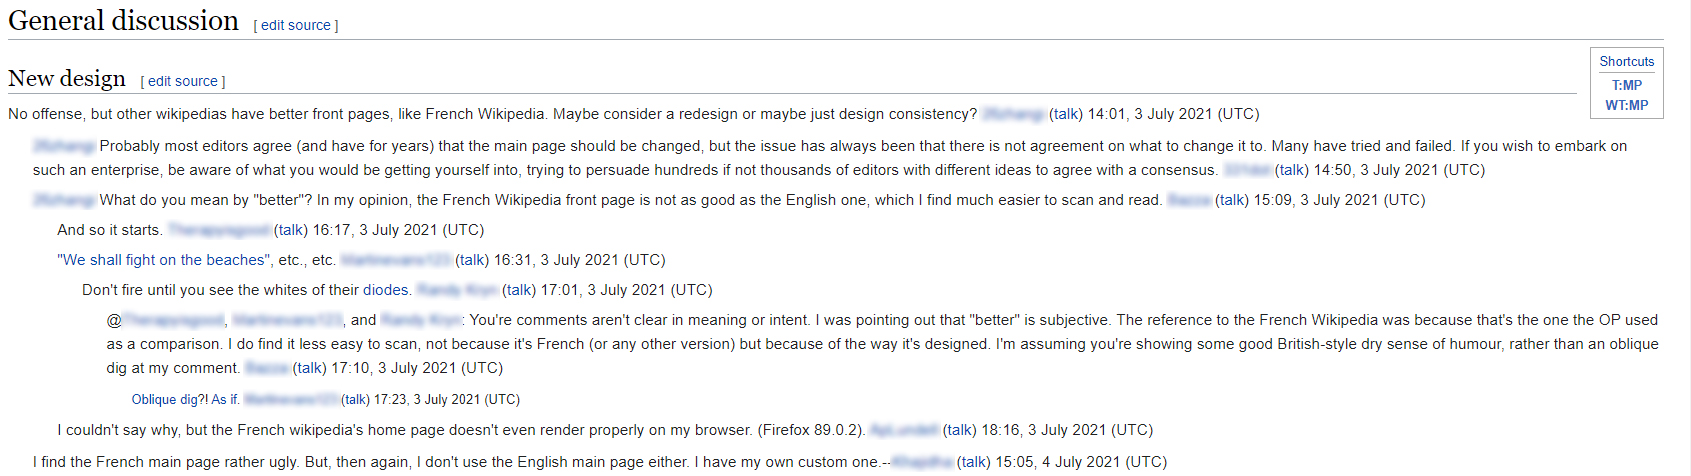
\includegraphics[width=1\textwidth]{./img/discussion.jpg}
    \caption{Example of a discussion on a talk page}
    \label{fig:discussion}
\end{figure}


\section{WikiConv Dataset}
\label{sec:wikiconvdataset}
WikiConv is a multilingual corpus encompassing the history of conversations on Wikipedia Talk Pages, including deletion, modification, and restoration of comments, called actions.\footnote{\url{https://github.com/conversationai/wikidetox/tree/main/wikiconv}} The version we used includes all conversations extracted from the 2020-01-04 Wikipedia dumps of English, Spanish, Italian, and Catalan.

Each language version of the dataset is split into smaller files compressed through gzip. The files contain an action for each line.

\begin{table}[H]
    \centering
    \ra{1.2}
    \begin{tabularx}{\columnwidth}{@{}Xrrrr@{}}
        \midrule
        \textbf{Language} & \textbf{Number of actions} & \textbf{Number of files} & \textbf{Size of files} & \textbf{Total size}\\ \toprule
        English & 235 Millions & 50 & 2.5 GB & 485 GB \\
        Spanish & 20 Millions & 5 & 2 GB & 41 GB \\
        Italian & 17 Millions & 5 & 2 GB & 41 GB \\
        Catalan & 2 Millions & 1 & 2 GB & 7 GB \\

         \bottomrule
    \end{tabularx}
    
    \caption{Size of the WikiConv Dataset in various languages.  \label{table:datasetsize}}
\end{table}

An edit of a page by a user is called revision, and can be represented by several action of four different kinds:

\begin{itemize}
\item \textbf{Creation}: An edit that creates a new section in a Wikipedia page.
\item \textbf{Addition}: An edit that adds a new post to a thread.
\item \textbf{Modification}: An edit that modifies an existing post.
\item \textbf{Deletion}: An edit that removes a post.
\item \textbf{Restoration}: An edit that restores a previously removed post.
\end{itemize}

Each action is a JSON object that contains several pieces of information, as listed on the dataset documentation. The most relevant data for this study is: the page title and page id; the user name and id; the text of the post underlying the action; the timestamp of the revision and the type of action.


\begin{figure}[H]
    \centering
    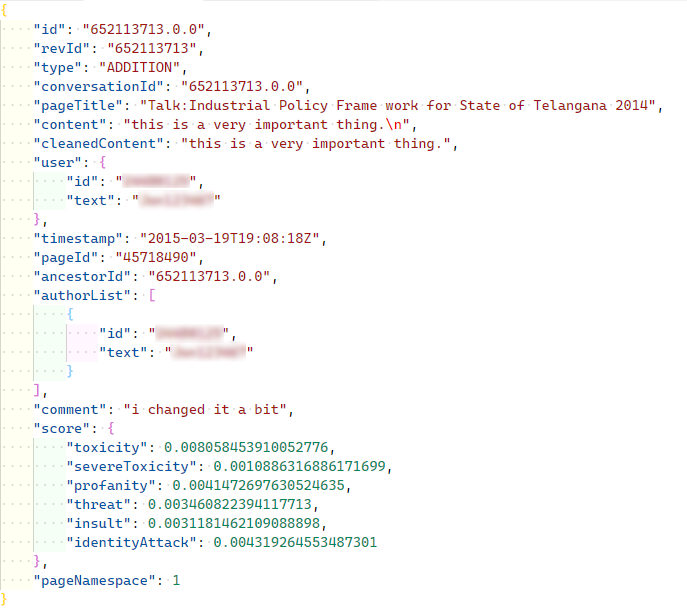
\includegraphics[width=0.7\textwidth]{./img/wikiconv.png}
    \caption{Example of an action contained in the English WikiCovn}
    \label{fig:wikiconv}
\end{figure}


\section{Emotional analysis}

Emotional analysis tries to understand which emotions a user expresses while writing. Thanks to the WikiConv dataset, we can analyze what users wrote on Wikipedia talk pages and try to figure out their emotions through emotional analysis.

The spectrum of human emotions can be categorized in several ways. We choose the classification introduced in “Classifying emotion: a developmental account”~\cite{zinck2008classifying}, which suggests four types of basic emotions: fear, anger, joy, and sadness. Another classification we used is the separation of emotions into two sentiments: positive and negative.

Thanks to premade emotional dictionaries, we can associate each word in a post to a set of emotions and sentiments. We took into consideration the results obtained by EmoLex and LIWC.

\subsection{EmoLex}
EmoLex, or NRC Word-Emotion Association Lexicon~\cite{mohammad2013nrc}, is a list of English words and their associations with eight basic emotions (anger, fear, anticipation, trust, surprise, sadness, joy, and disgust) and two sentiments (negative and positive).\footnote{\url{https://saifmohammad.com/WebPages/NRC-Emotion-Lexicon.html}} The annotations were manually done by crowd-sourcing, and it is available for free for academic purposes. It contains 14,182 words, and its contents have been translated in over 100 languages with Google Translate since it has been shown that a majority of effective norms are stable across languages. There are present the four languages we are interested in: English, Spanish, Italian, and Catalan.

\subsection{LIWC}
Linguistic Inquiry and Word Count (LIWC) associate words to psychologically relevant categories and is considered by many the “gold standard” of in computerize text analysis~\cite{tausczik2010psychological}.\footnote{\url{http://liwc.wpengine.com/}} To use LIWC an academic license is needed.

The latest LIWC dictionary was released in 2015 and consists of 6,400 words, linked to a set of relevant categories. LIWC is thought to be used through a processing module that takes as input a text and outputs percentages of different relevant categories it has found, but a dictionary file like the one offered by EmoLex can be extracted and used.

LIWC is available in different languages, including English, Spanish, and Italian. Currently, there is no version for the Catalan Language.

We got access to LIWC only in the last days of our research, and the results are not as thorough as the ones we got from EmoLex and are only used as validation.

      \chapter{Methods}
\label{cha:methods}
This project was part of a team effort. My contribution has been greatly influenced by other developers in our team, and the information we got were shared among us. For this reason, several aspects were a work of more than one person. In this chapter I will focus on what I personally did, but I will have to refer to work done in collaboration with others.

To share our projects and our implementations we used a GitHub organization where all our code can be found and used by others.\footnote{\url{https://github.com/WikiCommunityHealth}}

\section{Categorizing users}
\label{sec:categorizingusers}
Analyzing and making public data about a single user can be considered a violation of their privacy. We decided to group users into categories identified by their gender and role in Wikipedia and to publish only results relative to groups and not individuals.

Obtaining this information is not straightforward.

\subsection{Users' gender}
\label{sec:usersgender}
In Wikipedia, there are two main ways with which users can specify their genders: Userboxes and profile settings.

\subsubsection{UserBoxes}
\label{sec:usersboxes}
A UserBox, or UBX, is a graphical component that can be added to a user page. Some users have decided to express their gender through a corresponding UBX. There exist several genders related UBXs, grouped into 4 categories: “masculine”, “feminine”, “non-binary” and “others”.\footnote{\url{https://en.wikipedia.org/wiki/Wikipedia:Userboxes/Life/Gender}}

Thanks to Wikipedia APIs, we can list all pages that contain those templates, collecting a list of user pages, and thus usernames, that decided to express their gender as stated in the corresponding UBX.

As we will see in section \ref{sec:resuserboxes} this technique retrieved a relatively small amount of data if compared to profile settings.

\begin{figure}[H]
    \centering
    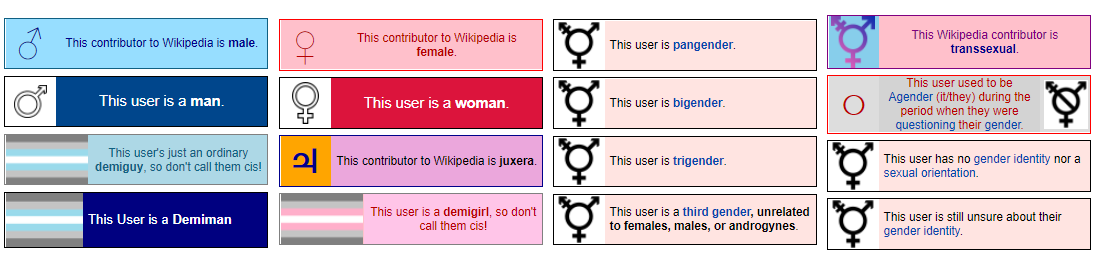
\includegraphics[width=0.85\textwidth]{./img/ubx.png}
    \caption{Examples of different UserBoxes used by the community}
    \label{fig:ubx}
\end{figure}

\subsubsection{Profile Settings}
\label{sec:profilesettings}
Each Wikipedia user has access to a settings page, where some preferences and information can be specified, including a user's gender. The user choice is restricted to “Male”, “Female” and “Unknown”, where “Unknown” is the choice selected by default when someone creates an account.

\begin{figure}[H]
    \centering
    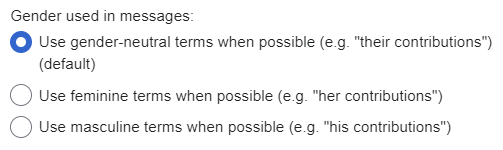
\includegraphics[width=0.7\textwidth]{./img/settings.png}
    \caption{Settings page where users can choose their gender}
    \label{fig:chainsuser}
\end{figure}

Wikipedia APIs returns a list of information about a user, among which their specified gender in the profile settings.\footnote{\url{https://www.mediawiki.org/wiki/API:Users}} We collected this and other information for all users for each language of Wikipedia.

\subsubsection{Users’ Role}
\label{sec:usersrole}
Users have been categorized based on their user groups. We considered the most common groups, which are Admins (or sysop), autopatrolled, and registered users.\footnote{\url{https://en.wikipedia.org/wiki/Wikipedia:User_access_levels}} This information has been retrieved from a dataset generated by another team member where all information about a user are collected, including their roles. Thanks to this dataset we could identify some users as a bot and remove them from our analysis.

\section{Lookup tables}
\label{sec:lookuptable}
The WikiConv dataset only provides information about actions. For our analysis, it was useful to have access to information about specific users and pages as a reference.

We decided to implement two lookup tables with basic information about each user and each page in a MongoDB instance,\footnote{\url{https://www.mongodb.com/}} a No-SQL database that stores data in JSON documents inside the collection. We choose this database because it allowed us to store and easily query our data without changing its format. To generate them, all the WikiConv dataset has been loaded into the database, then, a query, aggregated all information by the user and by page, and computed the new information seen in Figure \ref{fig:mongo}.

\begin{figure}[H]
    \centering
    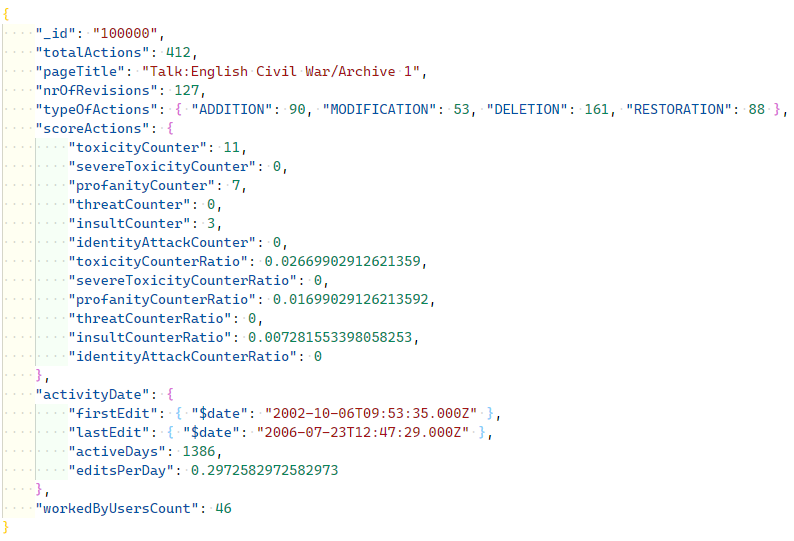
\includegraphics[width=0.85\textwidth]{./img/mongo.png}
    \caption{Examples of the document representing a Wikipedia page in the pages look-up table}
    \label{fig:mongo}
\end{figure}

\section{Sorting the WikiConv dataset}
\label{sec:sortingthewikiconvdataset}
The WikiConv dataset is composed of compressed files, each of them is about 2GB in size. Each file contains a random subset of actions of the entire dataset, and it is not possible to know in which file a specific action is contained.

We chose to sort the dataset in four different ways. Each sort is defined by a sorting feature. For each sorting feature, a set of intervals had to be chosen such that:
\begin{itemize}
\item  Each possible feature is part of one and only one interval.
\item  All intervals have a similar number of actions associated with them.
\item  All intervals are sorted such that if an interval is greater than another, then all its features are greater than the features of the other interval.
\end{itemize}

All the process was done by decompressing the file “on-the-fly”, without the need to store a plain version at any step of the process. This greatly increased performance, while reducing the storage space required for the process. The run time of the algorithm can be expressed as $O(N* M*log(M))$, where $N$ is the number of intervals, $M$ is the number of actions associated with an interval.

Of crucial importance was the choice of the dimensions of the intervals. An interval too big would result in a bigger $M$, a bigger file to sort, and thus a longer run time; whether a smaller interval would create a huge number of files to sort and a hardware bottleneck on the reading and writing performance, both during the sorting and during the analysis.

The four different sorting features are Users, Pages, Timestamp, and Reply-To.

\paragraph*{Users}
Each action can be associated with the user that made it, which can be identified by its numeric id. If an action was made by an anonymous user, no user id is saved on the dataset, but we can use its IP address to identify it. This method is not guaranteed to univocally identify a user, since many users can share the same IP address, or the same user can change IP address over time. A small set of actions had no user id and no IP address.

They were associated with a null user for the sake of the algorithm but were not analyzed after.

\paragraph*{Page}
To sort by page, we used the page id saved on each action as a sorting feature. The intervals are ranges of dimension 2 million, which covers all possible pages’ ids.


\paragraph*{Timestamp}
To sort by timestamp, we used the timestamp saved on each action. Actions from the same revision have the same timestamp, and we used their id as a secondary sorting feature since ids are ordered inside a revision. The intervals range from the start to the end of each month analyzed by the dataset.

\paragraph*{Reply To}
The reply to is a field that is not present in the original dataset. It was computed by another team member, by reconstructing the discussion tree of each page and assigning as “reply to”, the id of the user that the action was addressed to. This field is useful to understand which emotions are addressed to which user.

The intervals we used are the same as the ones we used for the user id.


\begin{table}[H]
    \centering
    \ra{1.2}
    \begin{tabularx}{\columnwidth}{@{}Xrrrr@{}}
        \midrule
        \textbf{Language} & \textbf{Lines} & \textbf{Size} & \textbf{Compressed size} & \textbf{Time to sort}\\ \toprule
        English & 235 Millions & 485 GB & 129 GB & 12 h \\
        Spanish & 20 Millions & 41 GB & 11 GB & 1:30 h \\
        Italian & 17 Millions & 41 GB & 11 GB & 1:30 h \\
        Catalan & 2 Millions & 7 GB & 2 GB & 0:30 h \\

         \bottomrule
    \end{tabularx}
    
    \caption{The table shows the number of actions in each dataset, the size of the compressed and uncompressed dataset and how much it took to compress.  \label{table:datasetsize}}
\end{table}


\section{Minifying the WikiConv dataset}
\label{sec:minifingthewikiconvdataset}
The WikiConv contains a lot of information that is not used during our analysis. We choose to generate a new parsed dataset containing only the information we needed. For each action, we kept id, action type, page title and id, username and id, and timestamp. The text content was parsed into an array of integers, where each integer is the number of words in the text associated with an emotion according to the lexicon dictionary.

Analyzing these versions of the dataset was much faster since the words were already associated to an emotion, and thanks to the reduced size of the file. It was also simpler to move and store the files.

\begin{figure}[H]
    \centering
    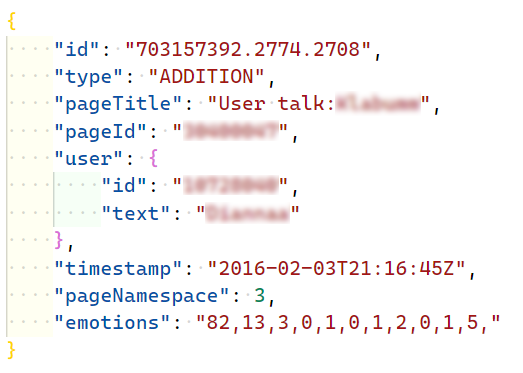
\includegraphics[width=0.6\textwidth]{./img/min.png}
    \caption{Examples of the document representing an action in a minified dataset}
    \label{fig:min}
\end{figure}


\begin{table}[H]
    \centering
    \ra{1.2}
    \begin{tabularx}{\columnwidth}{@{}Xrr@{}}
        \midrule
        \textbf{Language} & \textbf{Sorted dataset size} & \textbf{Minified dataset size} \\ \toprule
        English & 81 GB & 3.2GB  \\
        Spanish &  6.8 GB & 0.32 GB \\
        Italian &  6.1 GB & 0.30 GB \\
        Catalan &  1.4GB & 0.04 GB \\

         \bottomrule
    \end{tabularx}
    
    \caption{The table shows the difference in size from the sorted dataset to the minified dataset. \label{table:datasetsize}}
\end{table}


\section{Analyzing the WikiConv dataset}
\label{sec:analyzingthewikiconvdataset}
All the analysis tools have been written in Python 3.\footnote{\url{https://www.python.org/}} Python is an interpreted programming language suited for data science. It has a plethora of useful libraries for the tasks we are interested in and offers great flexibility.

We developed a python module that offers a command-line interface to allow a user to analyze either the sorted WikiConv dataset and the minified sorted WikiConv dataset. Through dependencies injection, the module can load an “analyzer”: a service that offers some APIs for the module to compute a different kind of analysis.

The module computes several tasks. Firstly, it reads a specified set of files, decompressing them on the fly, if necessary. Then it goes through all actions in the file, grouping them by their sorting feature. Since the sorting feature is sorted, once a different feature is read, the previous group is completed and can be passed as input to the analyzer which does its specific computations and remove from memory. The module also handles parallelization running each file in a different thread. The user can specify if he wants to use parallelization and the maximum number of parallel threads running.

An analyzer handles every possible analysis. They can be developed independently but need to implement a set of APIs called by the module. They are used to pass the actions groups and to synchronize the progress among different threads.

We developed several analyzers to handle different tasks, the important ones are described here:

\paragraph*{Minifier}
This analyzer allowed us to reduce the dataset structure as described in section \ref{sec:minifingthewikiconvdataset}. It took each line, calculated its minified version, and generated the new file version.

\paragraph*{Reply To}
It was used to create a new feature in the dataset called “replyTo” described in section \ref{sec:sortingthewikiconvdataset}. This feature identifies which users are an action addressed to.

\paragraph*{Reply To}
Mean and Var Analyzer:	It analyzed the mean and variance of emotions in each activity group. The output is a JSON file containing the total mean and variance of each emotion contained in the analyzed text and the number of actions analyzed. The results were also calculated and saved for each month contained in the action group. This gave us global information about a user or a page through time. It was also possible to use this analyzer to compute the same information for the whole dataset, giving us a reference point and a view of the whole Wikipedia in a particular month.

\paragraph*{Word Cloud}
Word Cloud:	This analyzer created a graphical representation of the most used words by a user, by a page, in a month, or Wikipedia as a whole. Seeing what words, the lexicon analyzed and associated with different emotions was difficult to verify manually, and having a graphical representation of its work was useful. It was used to verify and validate our works and the dataset we used and to illustrate our works to others simply and effectively.

\paragraph*{Emotions to DB}
This analyzer reads all emotions and generates the metrics to add to a Postgres database. We created metrics about pages and users’ groups for any month in the dataset. These metrics were saved in a SQL database and were then published.

\paragraph*{Emotions to JSON}
This analyzer, similarly to “Emotion to DB”, generates metrics about users’ groups and pages, but saves them in a JSON file. This is mostly used to rapidly share information among team members and is used as input for other scripts, such as the one that draws the charts.

\paragraph*{Emotions to CSV}
Similarly, to “Emotions to DB” and “Emotions to JSON”, this analyzer generated metrics about users’ groups and pages in CSV. These files were used by a researcher to develop a project of data visualization. We choose to use CSV since it is a simple and straightforward file format, that can be used without any special technical abilities.


\section{Metrics}
\label{sec:metrics}
Metrics are the core result of this study. They can be used to characterize users and pages by their emotions and can be exported and incorporated into other projects. It is important to make all metrics useful on their own and should be compared with each other. Each team member had different metrics and different approaches to compute them, but we tried to make them as similar as possible following this guideline:

\begin{itemize}
\item  Each metrics value should refer to a users’ group or a page
\item  Each metric value should refer to a month
\item  For each metric value there should be three linked metrics:
\begin{itemize}
\item  \textbf{Normalized}: the value normalized with a set of other metrics
\item  \textbf{Accumulated}: the current month metric value summed to all the same metrics of the previous months.
\item  \textbf{Accumulate Normalized}: the accumulated value normalized in the same way the normalize value was calculated.
\end{itemize}
\end{itemize}

To facilitate this process a Python package was developed, with the help of a team member. It helps our team members to format the metrics to follow our guidelines and push them into a database. The package can be installed via pip in any Python 3 project.


      \chapter{Results and Discussions}
\label{cha:results}

\section{Users' gender}
\label{sec:resusergender}
We retrieved information about a user gender in two ways: UsersBoxes and User’s settings. These data were then used to categories users’ in groups.

\subsection{UserBoxes}
\label{sec:resuserboxes}
Analyzing UserBoxes we retrieve relatively few data. Most Wikipedia users do not spend much time on their user page. To insert a UserBox it is required an effort by the user, that most are not willing to take. Gender UserBoxes allow a wide personalization and more can be added as needed. All genders are macro-categorized as Masculine, Feminine, Non-Binary and Other. 

\begin{table}[H]
    \centering
    \ra{1.2}
    \begin{tabularx}{\columnwidth}{@{}Xr@{}}
        \midrule
        \textbf{Genders categories} & \textbf{Number of users that used one of those UserBox} \\ \toprule
        Masculine & 10,489 Users  \\
        Feminine &  2,045 Users \\
        Non-Binary &  347 Users \\
        Other &  218 Users \\
        \bottomrule
        Total &  13,099 Users \\

         \bottomrule
    \end{tabularx}
    
    \caption{The table shows the number of users that implemented a UserBox of a particular category. \label{table:datasetsize}}
\end{table}

This approach may be subjected to some biases. Users that do not feel included in the limited gender selection of the Wikipedia user profile, may tend to express their identity through this feature, while users correctly represented on their settings, may not feel the need to use this feature. Another known bias, particularly on internet community, is the tendency, from female users, to not specify their gender or specify it as male. This is due to the fact that female users are subjected to discrimination in these platforms and tend to hide their true gender.

\begin{figure}[H]
    \centering
    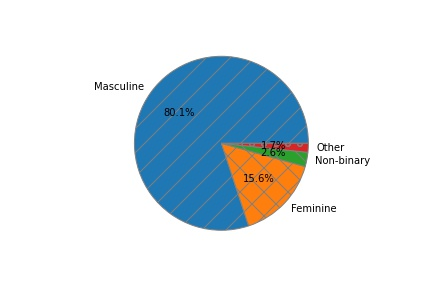
\includegraphics[width=0.6\textwidth]{./img/userbox.jpg}
    \caption{Percentage of editors with a UserBox for each gender group}
    \label{fig:userbox}
\end{figure}

We choose to not use this data, because it was statistically too small if compared to the profile settings and would generate groups to with few to no data at all.

\subsection{Profile settings}
\label{sec:resprofilesettings}
Profile settings is the most used feature to express a user gender. Its options are limited to male, female and unknown, where the unknown option is set by default. Most users never change this option, and are thus categorized as unknown, so, this specific label does not represent any valuable information.

This information is subjected to the same biases stated above, but it was the best we could do with the resources we had. Our results show a similar distribution of female and man to more accurate studies such as "Gender differences in Wikipedia editing" \cite{antin2011gender}. We can confidently say our results are a good representation of male and female users in Wikipedia.

We only needed data about English, Spanish, Italian and Catalan Wikipedias, but we decided to collect data for all Wikipedias. The results for the most common Wikipedia languages are shown in table 4.2.

\begin{table}[H]
    \centering
    \ra{1.2}
    \begin{tabularx}{\columnwidth}{@{}Xrrr@{}}
        \midrule
        \textbf{Wikipedia} & \textbf{Female Users} & \textbf{Male Users} & \textbf{All Users} \\ \toprule
        English & 122,445 & 604,633 & 40,526,936  \\
        Spanish & 30,774 & 106,269 & 6,071,869  \\
        German & 14,371 & 79,010 & 3,603,382 \\
        French & 9,275 & 48,531 & 3,968,600 \\
        Russian & 55,065 & 173,019 & 2,891,204 \\
        Italian & 7,731 & 39,037 & 2,060,494  \\
        Catalan & 1,499 & 5,145 & 373,672  \\

         \bottomrule
    \end{tabularx}
    
    \caption{The table shows the number female, male and total user for the most used Wikipedia. \label{table:datasetsize}}
\end{table}

This data was used in to generate two user groups: female and male.

We analyzed the gender distribution for users with different edits counts, since it is a simple way to identify a user level of activities, and it can be said that users with more edits are more active. The results are shown in Figure 4.2.

\begin{figure}[H]
    \centering
    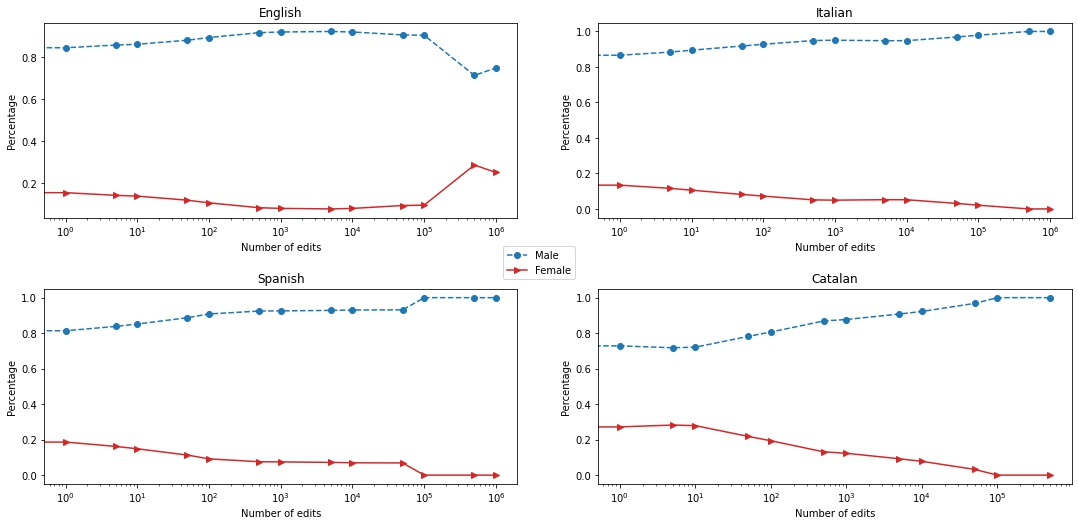
\includegraphics[width=0.95\textwidth]{./img/gedit.jpg}
    \caption{Percentage of male and female based on edit count, in four different Wikipedia. The users edit count is calculated based on a series of threshold, that a user can reach. The thresholds are: $0, 1, 5, 10, 50, 10^2, 5 \cdot 10^2, 10^3, 5 \cdot 10^3, 10^4, 5 \cdot 10^4, 10^5, 5 \cdot 10^5, 10^6$  }
    \label{fig:gedit}
\end{figure}

Our analysis compares male users and female users to a reference made by all users. All data have been shared in our group, but it was not made publicly available to avoid users’ privacy violations.

As seen in Figure \ref{fig:gedit} male editors are the vast majority of users, and the difference between male and female editors tend to grow with the edit count.


\section{Emotions}
\label{sec:resemotions}
Emotions are the core of this study. We analyzed the emotion expressed by users on the article and user talk pages. The analysis was done with EmoLex.

\begin{table}[H]
    \centering
    \ra{1.2}
    \begin{tabularx}{\columnwidth}{@{}Xrrr@{}}
        \midrule
        \textbf{WikiConv} & \textbf{Action analyzed} & \textbf{Words analyzed} \\ \toprule
        English & 4,163,088 & 1,178,703,180 \\
        Spanish & 469,051 & 95,987,997 \\
        Italian & 245,886 & 45,248,302 \\
        Catalan & 28,557 & 7,264,086 \\
         \bottomrule
    \end{tabularx}
    
    \caption{The table shows the number of actions and words analyzed foreach WikiConv Dataset during our analysis. \label{table:datasetsize}}
\end{table}

Our first result was to calculate how much each emotions was expressed in the language we analyzed. We estimated the percentage of words which express an emotion or a sentiment over all words analyzed that were contained in the emotion dictionary. The results are shown in Figure \ref{fig:emlang}.

\begin{figure}[H]
    \centering
    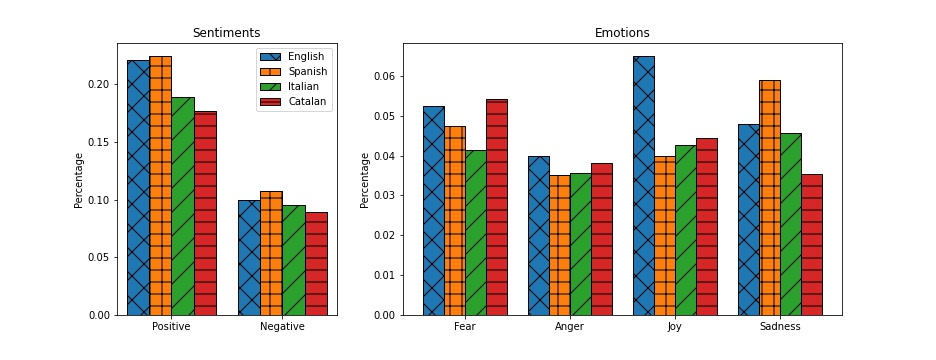
\includegraphics[width=0.95\textwidth]{./img/emlang.jpg}
    \caption{ The tables shows the percentage of emotions and sentiment expressed in all talk pages on different Wikipedia }
    \label{fig:emlang}
\end{figure}

\subsection{Word Clouds}
We analyzed a great quantity of data. It was necessary to have a visual representation of what we were doing. We choose to represents the most common words identified as emotions by our dictionaries in a "Word Cloud".\footnote{\url{https://amueller.github.io/word_cloud/}} Some sample results can be seen in Figure

\begin{figure}[H]
    \centering
    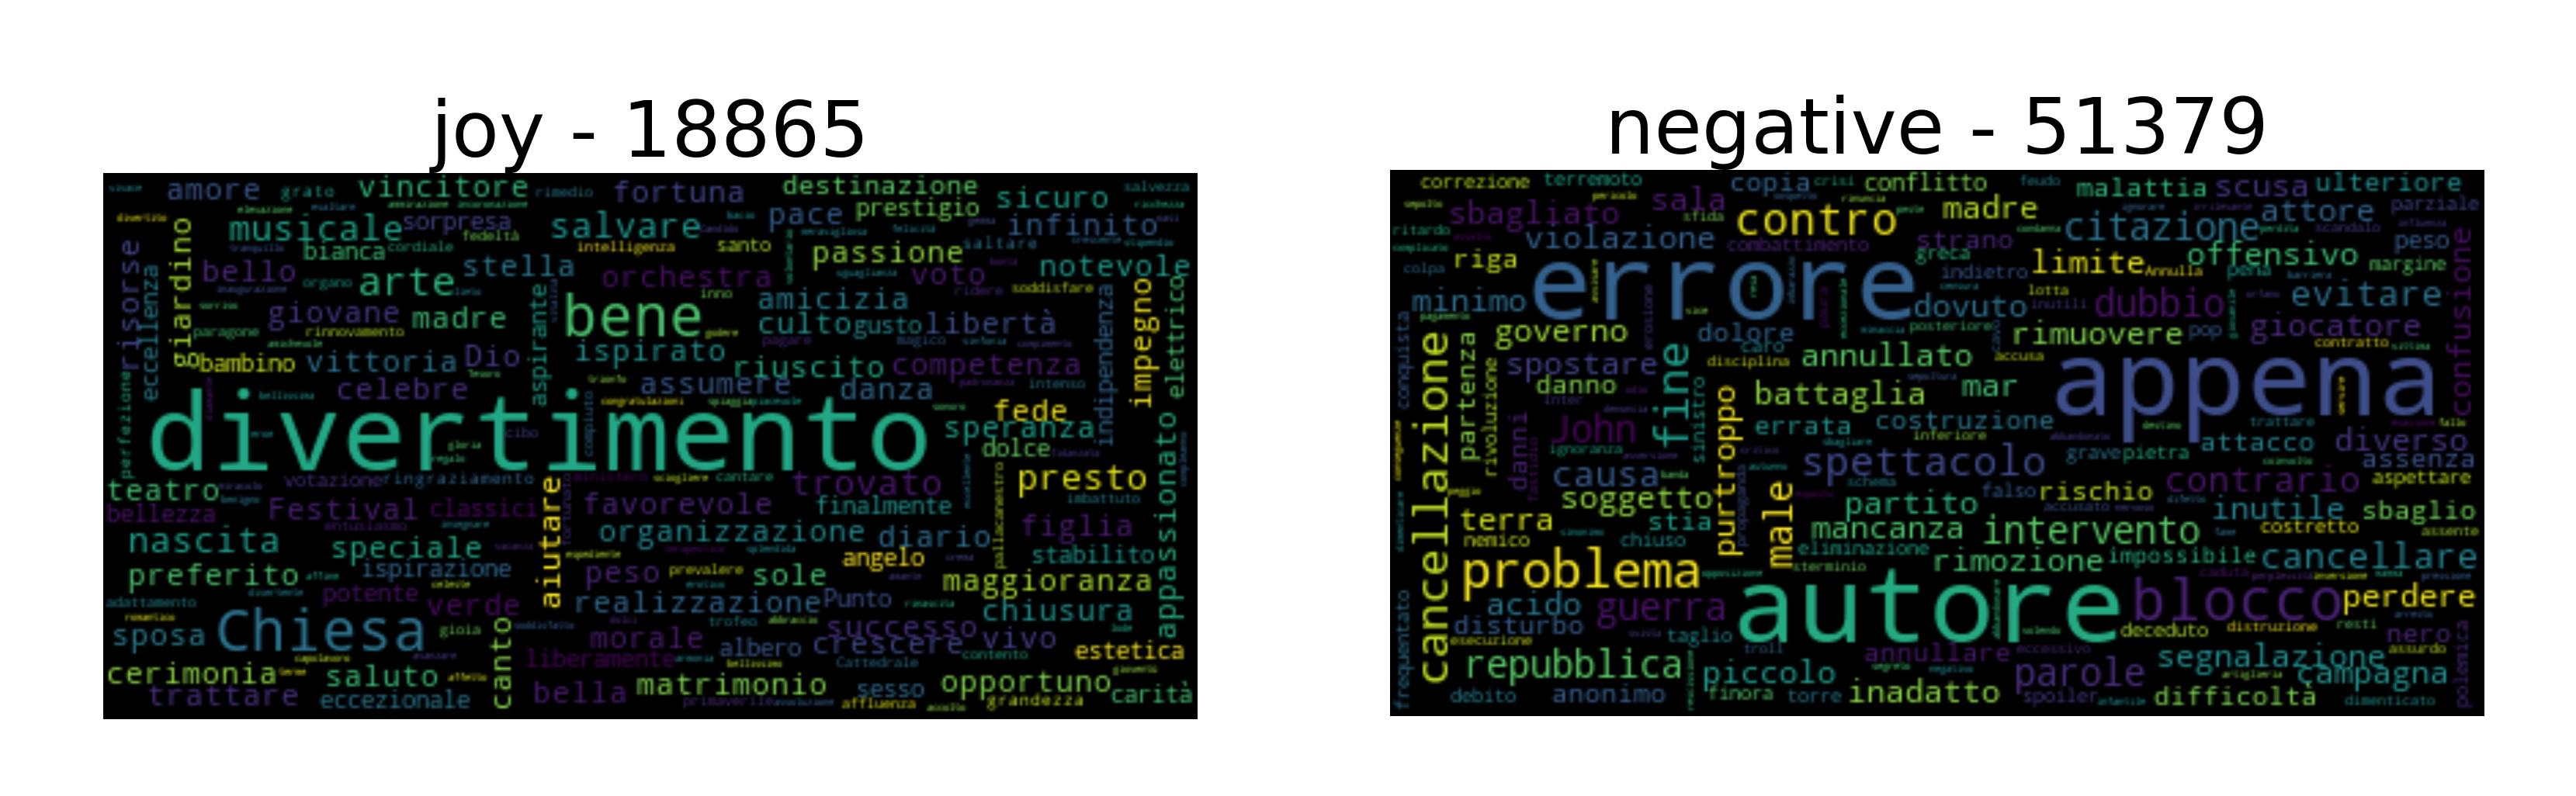
\includegraphics[width=0.95\textwidth]{./img/cloud.png}
    \caption{ This are two example of "Word Clouds" extracted from the Italian WikiConv of November 2019. The dimensions of a word in these images is directly related to their presence in the dataset. The number on the title is the total number of analyzed words that belong to that particular emotions. }
    \label{fig:cloud}
\end{figure}


\subsection{Users}
\label{sec:resusers}
We can use users' group previously defined to analyze their different emotional response. For each user we calculate the average value for the emotions over all its actions and averaged this with all other users in a group. The results can be seen in Figure \ref{fig:emgender} and Figure \ref{fig:emroles}.

\begin{figure}[H]
    \centering
    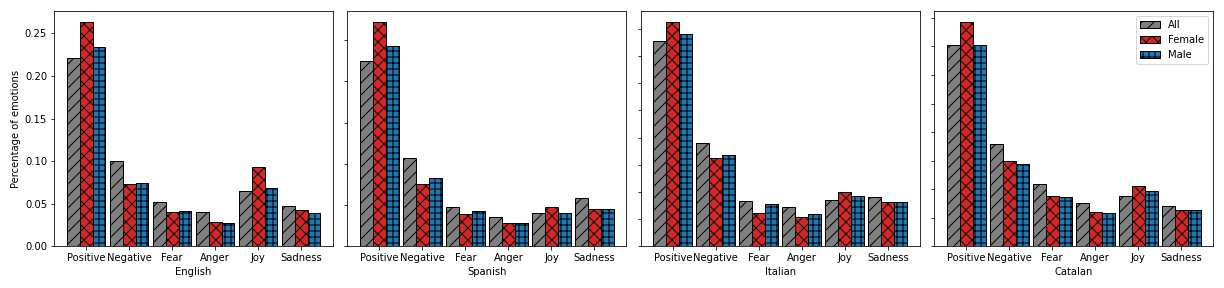
\includegraphics[width=0.95\textwidth]{./img/emgender.jpg}
    \caption{ The tables shows the percentage of emotions and sentiment expressed by female, male or all users }
    \label{fig:emgender}
\end{figure}

\begin{figure}[H]
    \centering
    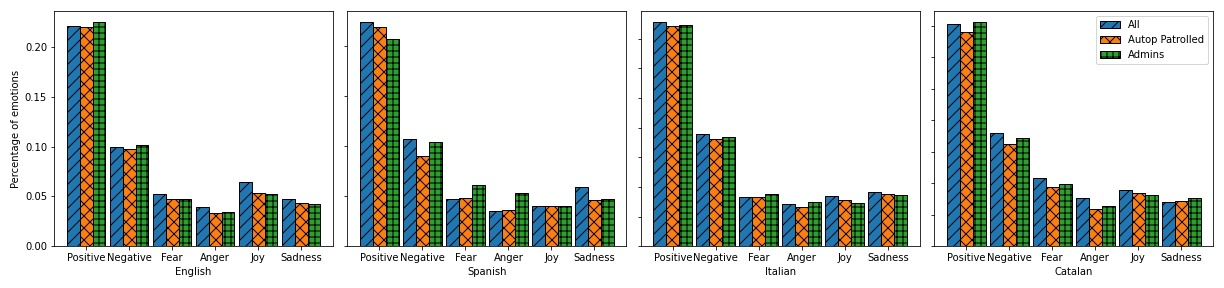
\includegraphics[width=0.95\textwidth]{./img/emroles.jpg}
    \caption{ The tables shows the percentage of emotions and sentiment expressed by admins, auto patrolled and for all user }
    \label{fig:emroles}
\end{figure}

In figure \ref{fig:emgender} we can see that female editor have a tendency to express more positive sentiment than male. This is was also show in previous studies \cite{laniado2012emotions} \cite{iosub2014emotions}.

We are interested in users life-cycles, from when they join Wikipedia to the moment they leave. To better understand how users feels during their life as a Wikipedia editor we analyzed all emotions they express. We took an average of a user action in each month after their complete their first action, and averaged them with all users in a group or with all Wikipedia's users. We took into consideration that the number of active users decrees over time. We also analyzed the emotions a user received from others.

\begin{figure}[H]
    \centering
    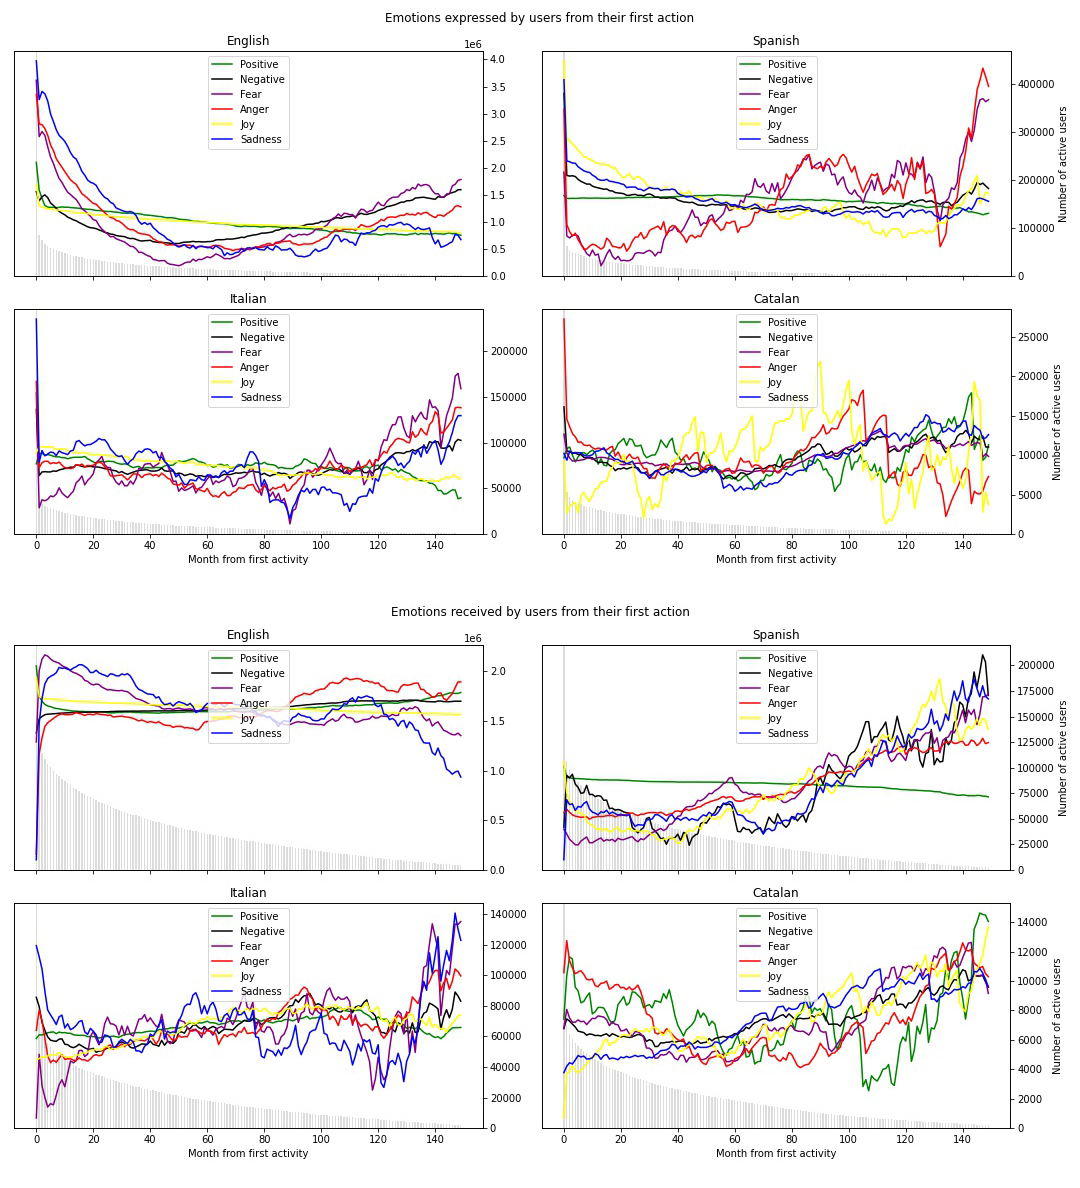
\includegraphics[width=1\textwidth]{./img/mstart.jpg}
    \caption{ The two tables shows the normalized value of each emotion and sentiment analyzed for four languages.  The bars in the background represent the number of active users it and the x axis are the month from a user first activity. The first table shows the emotions expressed by a users in they actions and the second the emotions received through reply to their posts. }
    \label{fig:mstart}
\end{figure}

Life-cycles can also be analyzed for different users' groups and compared between them. This can be useful to understand differences between different users.

\begin{figure}[H]
    \centering
    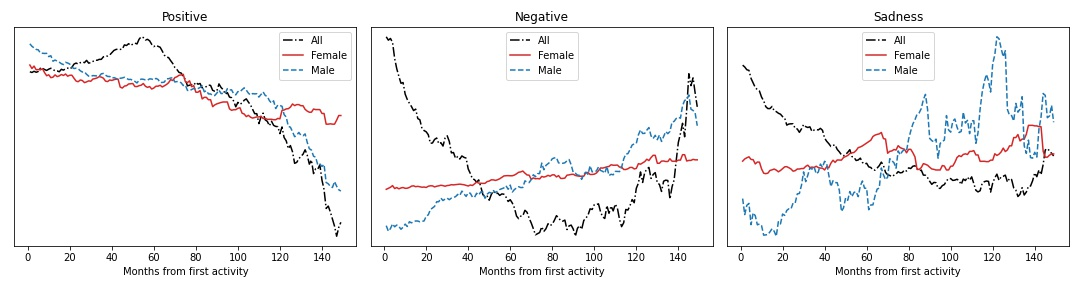
\includegraphics[width=0.9\textwidth]{./img/gtime.jpg}
    \caption{ The two tables shows the normalized value of different positive, negative and sad words used by users of different gender from their first action. }
    \label{fig:gtime}
\end{figure}

To understand how external events influence users on Wikipedia it is useful to see variation of emotions over time. For this reason we analyzed user emotions for over each month from the opening of Wikipedia, in a similar way we analyzed user life-cycle. It is important to remember that, in the early days Wikipedia was less used, and we have less data. Wikipedia reached a good level of popularity around 2007.

\begin{figure}[H]
    \centering
    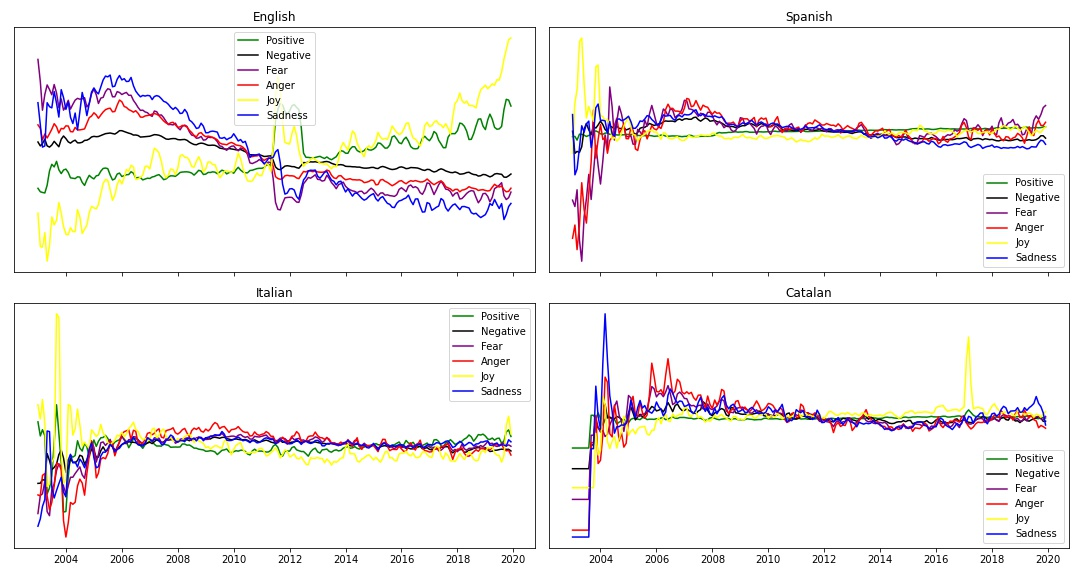
\includegraphics[width=0.9\textwidth]{./img/time.jpg}
    \caption{ The table shows the normalized value of all analyzed emotions over time. The emotions are sampled each month }
    \label{fig:time}
\end{figure}

\subsection{Pages}
\label{sec:respages}
Pages were analyzed similarly to users. In this case there were less privacy concerns since pages aggregate contribution from different users. We did not made any groups of pages. Smaller pages do not have enough information to be considered statistically useful, but bigger pages could be analyzed. Since it did not increase significantly our calculation time, we decided to analyze all pages and save the metrics we generated to our database.

Every page has a metric for each emotion and sentiment from any month of its life.

\begin{figure}[H]
    \centering
    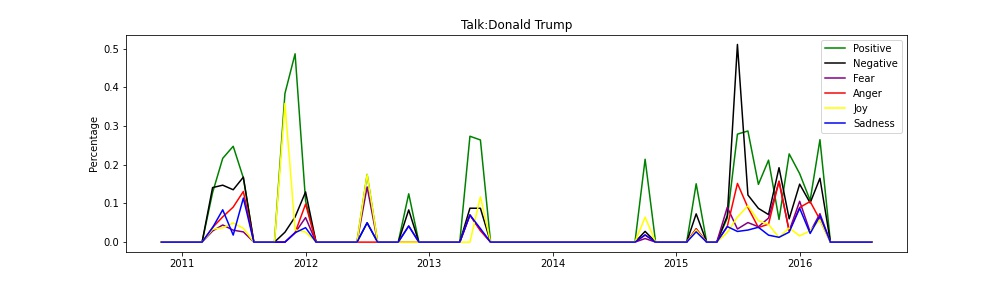
\includegraphics[width=1\textwidth]{./img/trump.jpg}
    \caption{ The table shows the emotions expressed by editors on the talk page of the article related to Donald J. Trump }
    \label{fig:trump}
\end{figure}

      \chapter{Infrastructure}
\label{cha:infrastructure}

\section{Storing the dataset}
\label{sec:storingthedataset}
We stored the dataset in multiple ways, each better suited for different tasks.

The original WikiConv, its four sorted copies, and the relative minified versions were stored as compressed gzip files on a hard disk and backed up in Google Drive. This hard drive was accessible from all the computers we used to perform the analysis.

A copy of the original dataset was decompressed and loaded in a MongoDB instance, where the look-up table was also created. MongoDB is a non-relational database that uses a JSON structure for its data, making it a good fit for the WikiConv data structure. It was used to launch simple queries on the dataset and retrieve immediate results. MongoDB was also useful for other related projects, which used our data in their analysis, and could easily use it.

\section{Storing our results}
\label{sec:storingourresults}
Results are stored in four ways: A Postgres database,\footnote{\url{https://www.postgresql.org/}} A mongoDB instance, JSONs files and CSVs files.

Among all members of our group, we choose to use a similar format for all our metrics. All the relevant metrics we generated can be saved in a Postgres database and do not contain sensitive information. Each Table collects information about a single language analyzed. The rows every month are analyzed for each page and user group.

MongoDB was mostly used for the look-up tables. It was also used to extract the information needed during our analysis that was made by other team members and was stored on a MongoDB instance.

JSON files were used to save simple results, that could be shared or used to plot charts.

CSV files were mostly used to save data used in our analysis that did not need to be loaded to a proper database and needed to be read quickly from a file. This is also the format the emotion EmoLex used.

\section{Public API}
\label{sec:publicapi}
We want to make publicly available the metrics we calculated, but the dataset is large and, usually, only a small portion of it is necessary for any related work. Forcing people to load the whole dataset can be time-consuming and take up lots of resources, setting a high bar for anybody interested in using our data. To reduce this stress, we decided to make a public API endpoint. People can now query our dataset without the need to install it on their machine and retrieve only the information they need.

To maximize the flexibility of our APIs results, we implemented GraphQL, a query language made for APIs.\footnote{\url{https://graphql.org/}} It allows users to write and send to our backend their query. We can validate and execute their request and return the data in the format they asked for. GraphQL also offers a landing page, reachable from any browser where user can compose their query and are helped by the UI to understand our database structure.

To link GraphQL to our Postgres database we used Hasura, a software that automatically maps a Postgres database to GrapQL. This solution allowed us to use GraphQL, without the need to implement a custom backend. We configured Hasura to allow anybody to read our data, but without the possibility to alter it.\footnote{\url{https://hasura.io/}}

\begin{figure}[H]
    \centering
    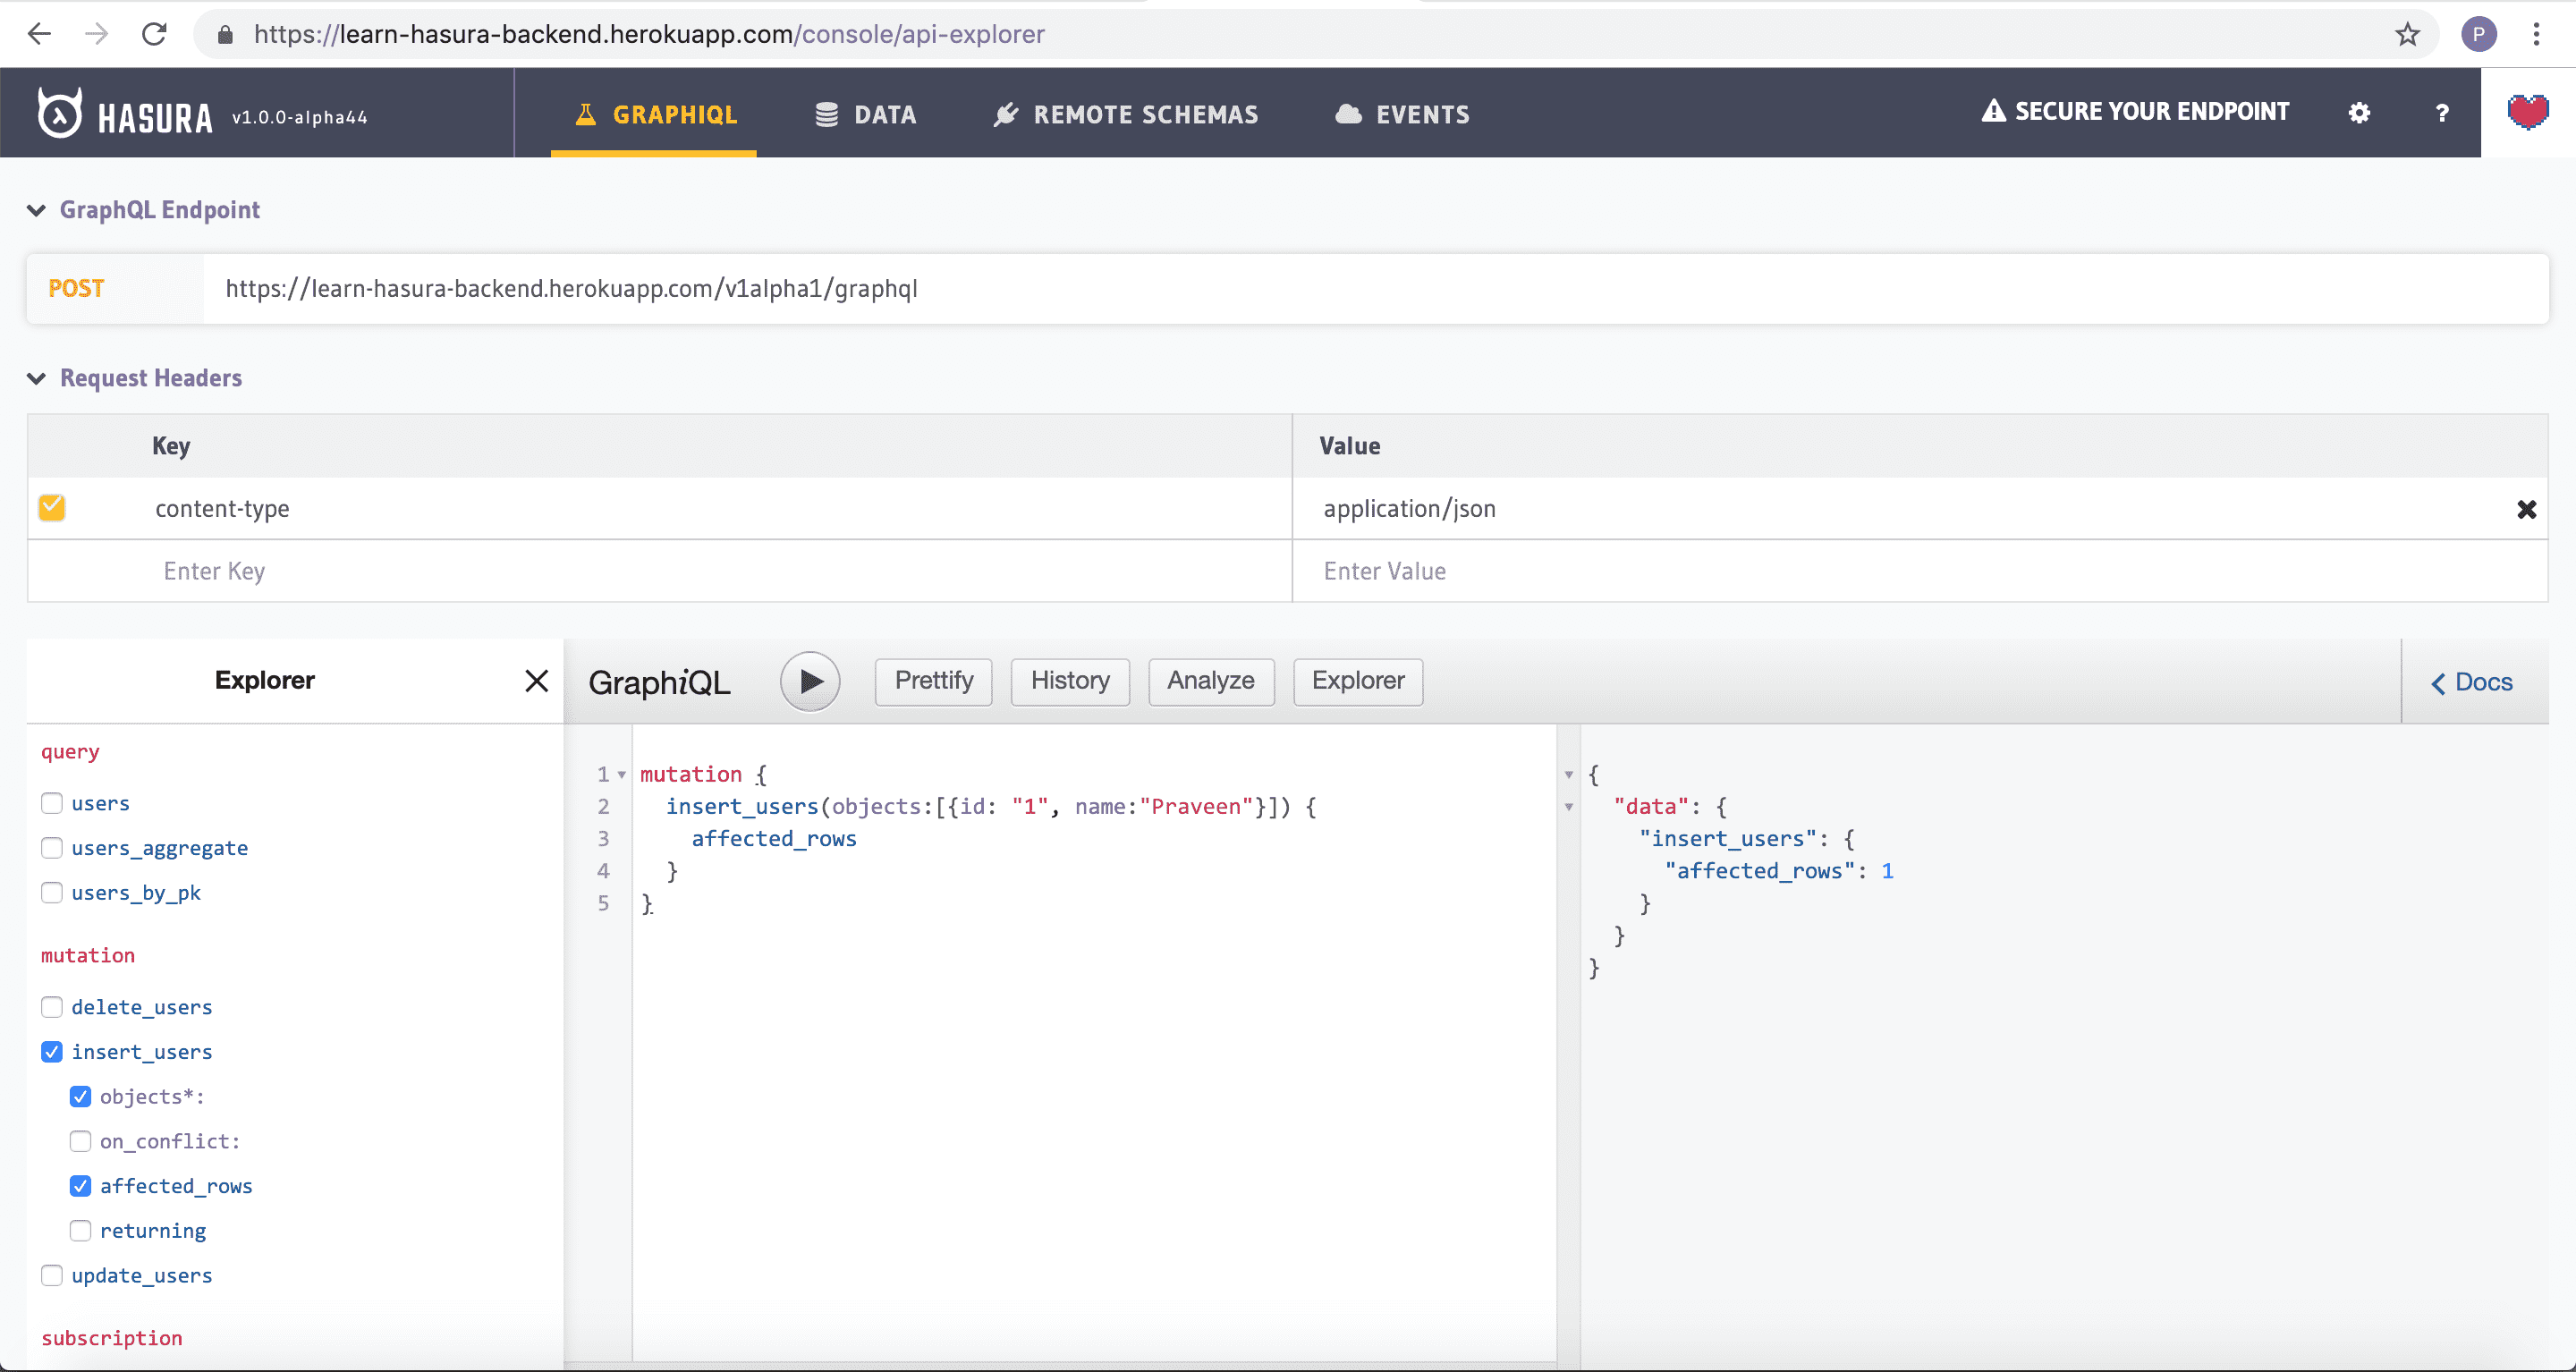
\includegraphics[width=0.8\textwidth]{./img/hasura.png}
    \caption{Hasura landing page, where a user can query our database}
    \label{fig:hasura}
\end{figure}

\section{Web Application}
\label{sec:webapplication}
We developed a web application to show chart combining multiple metrics. This application was developed in TypeScript\footnote{\url{https://www.typescriptlang.org/}} using the Vue.js framework.\footnote{\url{https://vuejs.org/}} For the charts we used the JavaScript version of Plotly.\footnote{\url{https://plotly.com/javascript/}}

The Web application provides a simple and accessible tool for anybody that wants to read and plot out metrics. It is accessible from a browser, and through a graphical user interface allows users to select which metrics to plot and compare. Thanks to the metrics being saved similarly, results from multiple projects from our team can be implemented.

The web application was developed in Typescript using Vue.js 3, a progressive JavaScript Framework. All code developed in Vue.js runs on the user browser, avoiding the need for us to maintain a complex infrastructure active, it is only required to serve the static HTML and JavaScript files from the server. To retrieve the data needed by a user, the web application queries the Hasura instance. This is done through Apollo,\footnote{\url{https://www.apollographql.com/}} a GraphQL implementation for Vue.js.

The charts were made with Plotly JavaScript, a charting library, which allows us to build complex charts with a high-level implementation. Charts show different metrics simultaneously and can be personalized by users.

\begin{figure}[H]
    \centering
    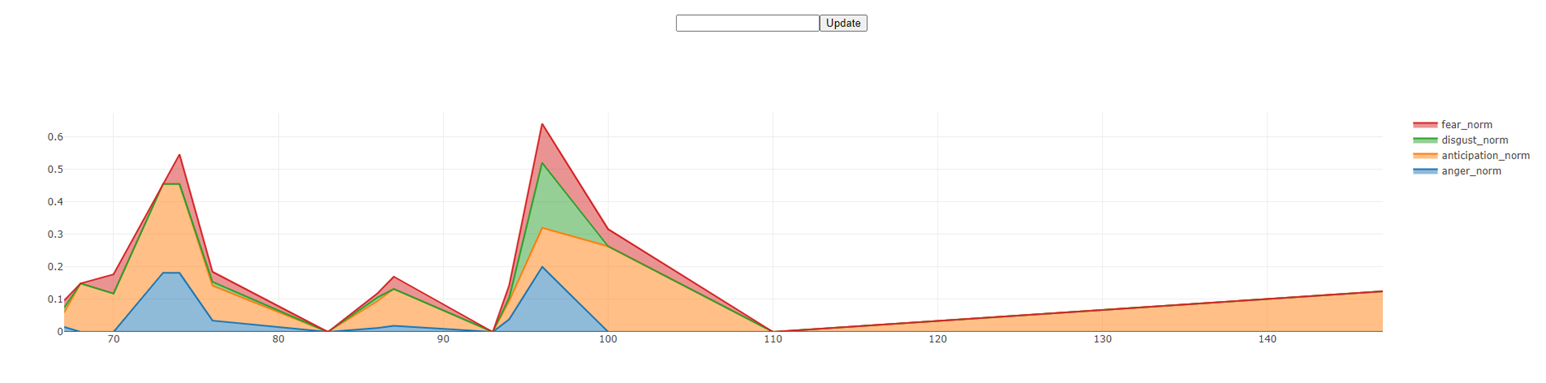
\includegraphics[width=0.95\textwidth]{./img/app.png}
    \caption{A page of the web app where a chart is showing severla metrics chosed by a user}
    \label{fig:chainsuser}
\end{figure}

\section{Deploy}
\label{sec:deploy}
To deploy our solution, we decided to use Docker.\footnote{\url{https://www.docker.com/}} It is a software that uses virtualization technology to deliver software in packages called container. Containers are isolated from one another and bundle their own software. Thanks to this technology we can deploy our database, Hasura, and our web application in three different containers. We can deploy our solution without worries about dependencies and compatibility, moreover, all our software is isolated and can be updated with continuous integration.

The Hasura container is public and anybody can implement their application using our data.

\begin{figure}[H]
    \centering
    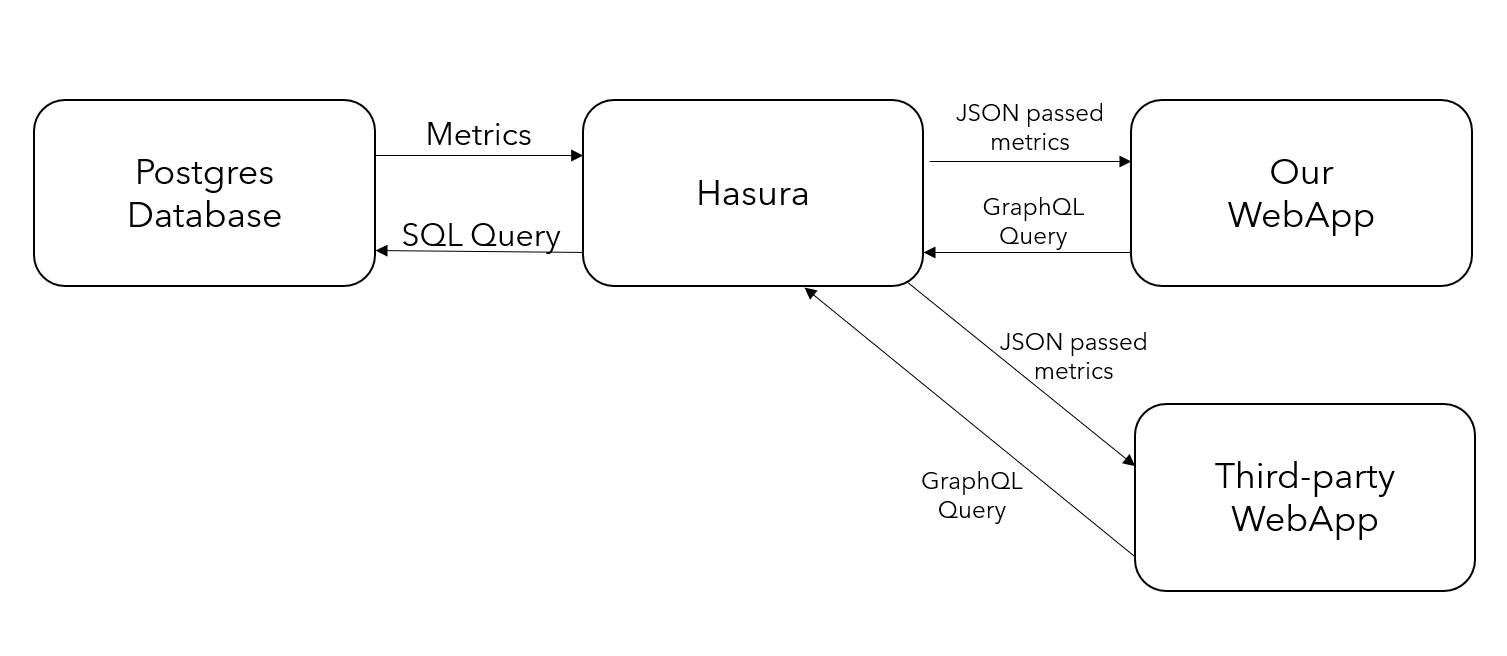
\includegraphics[width=0.80\textwidth]{./img/docker.png}
    \caption{This is a graphical rappresentations of out docker containers and a possible third-party application with their communication}
    \label{fig:docker}
\end{figure}

      \chapter{Conclusions}

With this project we have an overview of emotions expressed in Wikipedia discussions, but much more can be done. With the help of other team members, we plan to join our metrics and generate a better representation of an editor's life cycle. Future work on emotions can also be done. We want to implement other emotion lexicon, such as LIWC, to have a comparison with other system, and use information from other team members to better define users' group.

The current dashboard is a bare-bone version of what we have in mind. We want to keep improving it, joining metrics from different projects and giving users greater freedom on the choice of data thy want to visualize.

All the information we gather will soon be outdated. For this reason we are implementing a system that automatically updates our metrics with the latest Wikipedia dump. We also plan to extend this analysis to other languages.

All the code wrote, is public and was made to be modular, giving the possibility to others to continue this work.

      
      
    \endgroup


    % bibliografia in formato bibtex
    %
    % aggiunta del capitolo nell'indice
    \addcontentsline{toc}{chapter}{Bibliografia}
    % stile con ordinamento alfabetico in funzione degli autori
    \bibliographystyle{plain}
    \bibliography{biblio}
%%%%%%%%%%%%%%%%%%%%%%%%%%%%%%%%%%%%%%%%%%%%%%%%%%%%%%%%%%%%%%%%%%%%%%%%%%
%%%%%%%%%%%%%%%%%%%%%%%%%%%%%%%%%%%%%%%%%%%%%%%%%%%%%%%%%%%%%%%%%%%%%%%%%%
%% Nota
%%%%%%%%%%%%%%%%%%%%%%%%%%%%%%%%%%%%%%%%%%%%%%%%%%%%%%%%%%%%%%%%%%%%%%%%%%
%% Nella bibliografia devono essere riportati tutte le fonti consultate 
%% per lo svolgimento della tesi. La bibliografia deve essere redatta 
%% in ordine alfabetico sul cognome del primo autore. 
%% 
%% La forma della citazione bibliografica va inserita secondo la fonte utilizzata:
%% 
%% LIBRI
%% Cognome e iniziale del nome autore/autori, la data di edizione, titolo, casa editrice, eventuale numero dell’edizione. 
%% 
%% ARTICOLI DI RIVISTA
%% Cognome e iniziale del nome autore/autori, titolo articolo, titolo rivista, volume, numero, numero di pagine.
%% 
%% ARTICOLI DI CONFERENZA
%% Cognome e iniziale del nome autore/autori (anno), titolo articolo, titolo conferenza, luogo della conferenza (città e paese), date della conferenza, numero di pagine. 
%% 
%% SITOGRAFIA
%% La sitografia contiene un elenco di indirizzi Web consultati e disposti in ordine alfabetico. 
%% E’ necessario:
%%   Copiare la URL (l’indirizzo web) specifica della pagina consultata
%%   Se disponibile, indicare il cognome e nome dell’autore, il titolo ed eventuale sottotitolo del testo
%%   Se disponibile, inserire la data di ultima consultazione della risorsa (gg/mm/aaaa).    
%%%%%%%%%%%%%%%%%%%%%%%%%%%%%%%%%%%%%%%%%%%%%%%%%%%%%%%%%%%%%%%%%%%%%%%%%%
%%%%%%%%%%%%%%%%%%%%%%%%%%%%%%%%%%%%%%%%%%%%%%%%%%%%%%%%%%%%%%%%%%%%%%%%%%
    

    % \titleformat{\chapter}
    %     {\normalfont\Huge\bfseries}{Allegato \thechapter}{1em}{}
    % sezione Allegati - opzionale
    % \appendix
    % \input{allegati}

\end{document}
